\chapter{Motor}
\label{cap:p2}

O \textit{engine} tem como principal função apresentar o modelo gráfico. Para
tal utiliza-se a biblioteca \textit{GLUT (OpenGL Utility Toolkit )}, em conjunto com
a biblioteca gráfica \textit{OpenGL}.


\section{Objectivos}

Com o motor pretende-se que uma aplicação que seja capaz de ler um conjunto de pontos especificados em ficheiros '.3d' que estão indicados num ficheiro '.xml' e os desenhe numa janela. Além desse objetivo principal foi incluída uma câmara em torno do objeto desenhado e um pseudo-menu simples que permite alterar o modo de visualização dos pontos.

Nesta secção apresenta-se de que forma o motor foi desenvolvido, começando-se por explicar a leitura dos ficheiros

\section{Leitura Ficheiros}

\subsection{Ficheiro XML}

A estrutura do ficheiro XML contempla apenas dois tipos de elementos:

\begin{itemize}
	\item[\textbf{scene}] - elemento pai
	\item[\textbf{model}] - elemento com 1 atributo \textit{file} cujo valor corresponde ao nome de um ficheiro de pontos
\end{itemize}



O pseudo-codigo da função de leitura do XML pode ser expresso da seguinte forma:

\begin{Verbatim}

if(xml = fopen(argv[1],"r")) {
lê a primeira linha, verifica abertura do scene
while(consegue ler do xml) {
procura os model files e guarda os nomes 
}
fclose(xml);

} else {
perror(Impossivel abrir XML);}
}
\end{Verbatim}

\subsection{Ficheiros .3d}


Nos ficheiros '.3d', cada linha representa um ponto. Em cada linha exceto a primeira, existem 3 valores, separados por ponto e vírgula, correspondentes às coordenadas cartesianas do ponto. É necessário por isso ter uma função que seja capaz de ler os pontos destes ficheiros para que o motor os possa desenhar.

No main está um pedaço de código que permite a leitura destes ficheiros, que recebe como parâmetro o nome de um ficheiro e coloca os pontos lidos num vector de pontos ( variável global). Este vector de pontos será depois relido pelo \textit{rendeScene()} para desenhar os pontos.

A parte do código que lê o ficheiro '.3d' funciona da seguinte forma:


\begin{Verbatim}

while(existem nome de ficheiros para ler) {
  if(abre ficheiro para leitura) {
    if(verts = le a primeira linha para saber quantos pontos 
	tem de ler) {
      if (consegue reallocar mais memoria para o
        buffer(_buffer_pontos)) {
			
          for(k=primeiro lugar livre;(k < _buffer_size) &&
           (consegue ler o ponto);k++){
            pt = criaPonto()
            armazena o ponto no vector }
      } else {
        assinala o erro - (memoria/leitura/etc)
      }
    }
    fclose(f);
  } else {
      perror("cannot open file");
  }
  Incrementa o número de ficheiros lidos
}
 
 
\end{Verbatim}

\section{Desenho dos pontos}

O resultado da leitura do XML e dos ficheiros '.3d' nele especificados é um conjunto de \textit{Ponto3D} que são armazenados numa variável global. Este conjunto de pontos está implementado sobre a forma de um \textit{array<sPonto3D>}. 

A ordem pela qual os pontos aparecem no vector é a ordem pela qual apareceram nos ficheiros, que por sua vez é a ordem pela qual deverão ser desenhados. Nesta situação, desenhar os pontos corresponde simplesmente a percorrer todos os pontos colocados no \textit{array} e pedir ao GLUT para os desenhar. Mostra-se um excerto de código da função \textit{renderScene()} que corresponde ao desenho dos pontos:

\begin{Verbatim}

glBegin(GL_TRIANGLES);
glColor3f(0.0, 0.0, 1.0);

for(i = 0;i < _buffer_size;i++){
glVertex3f(_buffer_pontos[i].x,_buffer_pontos[i].y,
_buffer_pontos[i].z);
}

glEnd();
\end{Verbatim}



\section{Câmara}

Para se poder ver o objeto desenhado de vários ângulos foi implementada uma câmara.  
À função \textit{gluLookAt()} são passados argumentos que controlam a sua posição, onde estão focadas; a posição de \textit{up} nunca muda. 

\begin{Verbatim}
gluLookAt(xcam, ycam, zcam,
xcam+lx, ycam+ly,  zcam+lz,
0.0f, 1.0f,  0.0f);
\end{Verbatim}

É possível ao utilizador mudar a posição da câmara. Os controlos são os seguintes:

\begin{itemize}
	\item[\textbf{Tecla 'UP'}] permite ao utilizador fazer zoom in
	\item[\textbf{Tecla 'DOWN'}] permite ao utilizador fazer zoom out
	\item[\textbf{Tecla 'LEFT'}] permite ao utilizador arrastar a câmara para esquerda
	\item[\textbf{Tecla 'RIGHT'}] permite ao utilizador arrastar a câmara para direita
	\item[\textbf{Tecla 'Q'}] permite ao utilizador arrastar a camara para cima
	\item[\textbf{Tecla 'E'}] permite ao utilizador arrastar a camara para baixo 
	\item[\textbf{Tecla 'A'}] permite ao utilizador mudar o ponto de foco para a esquerda
	\item[\textbf{Tecla 'S'}] permite ao utilizador mudar o ponto de foco para baixo
	\item[\textbf{Tecla 'D'}] permite ao utilizador mudar o ponto de foco para a direita
	\item[\textbf{Tecla 'W'}] permite ao utilizador mudar o ponto de foco para cima

\end{itemize}



Quando a função \textit{gluLookAt()} é chamada e acede aos valores de x, y e z da posição da câmara, estes estão atualizados.

\section{Pseudo-Menu}

Para proporcionar alguma flexibilidade na visualização das figuras desenhadas foi incluído um menu que permite ao utilizador alternar entre o modo de visualização de pontos, linhas, ou objeto preenchido:

<<<<<<< Updated upstream
=======
\begin{figure}[htpb]
	\centering
	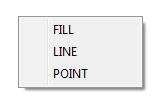
\includegraphics[scale=1.0]{imagens/p1_menuOpcoes.png}
	\caption{Menu de opções de visualização. Acessível com clique no botão direito do rato}
	\label{p1:fig:p1_menuOpcoes}
\end{figure}
>>>>>>> Stashed changes

O pseudo-menu foi pensado da seguinte forma:

\begin{itemize}
	\item[\textbf{Tecla 'F'}] permite ao utilizador alterar o modo do poligono para preenchido
	\item[\textbf{Tecla 'G'}] permite ao utilizador alterar o modo do poligono para linhas
	\item[\textbf{Tecla 'H'}] permite ao utilizador alterar o modo do poligono para pontos
\end{itemize}






<<<<<<< Updated upstream
=======
\begin{figure}[htpb]
	\centering
	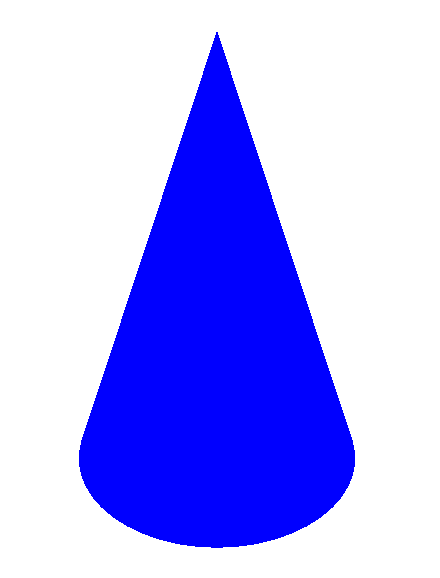
\includegraphics[scale=0.2]{imagens/p1_fill.png}
	\caption{Exemplo de cone construído no modo GL\_FILL}
	\label{p1:fig:p1_fill}
\end{figure}

\begin{figure}[htpb]
	\centering
	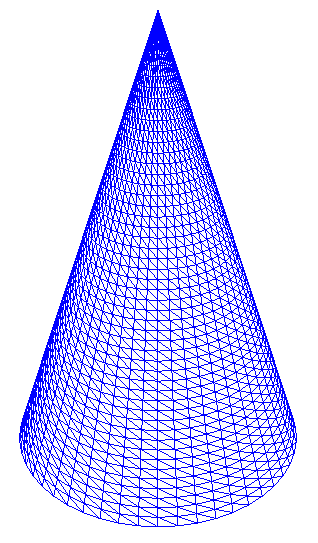
\includegraphics[scale=0.2]{imagens/p1_line.png}
	\caption{Exemplo de cone construído no modo GL\_LINE}
	\label{p1:fig:p1_line}
\end{figure}

\begin{figure}[htpb]
	\centering
	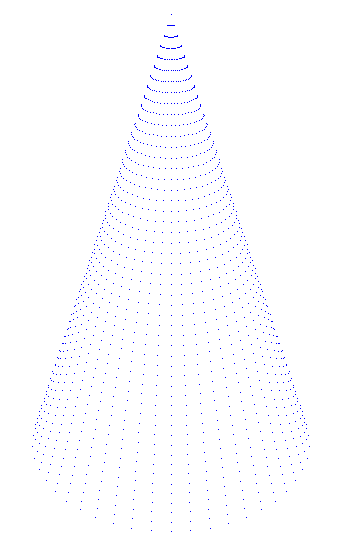
\includegraphics[scale=0.2]{imagens/p1_point.png}
	\caption{Exemplo de cone construído no modo GL\_POINT}
	\label{p1:fig:p1_point}
\end{figure}
>>>>>>> Stashed changes



